\singlespacing
To further compress the peak memory footprint, we first introduced three meta-heuristic algorithms—Local Search, Simulated Annealing (SA), and Genetic Algorithms (GA) to deeply optimize the initial solutions generated by the Greedy by Size method. During this phase, to facilitate rigorous research and analysis, we developed an automated hyperparameter tuning program and an intuitive memory allocation visualization tool. However, a critical observation emerged during the optimization process: the unoptimized Hole-aware Greedy algorithm would occasionally discover exceptionally superior solutions, outperforming even the heavily optimized Greedy by Size configurations, as shown in Table 2. 
\begin{table}[t]
\centering
\caption{Peak memory comparison on a fork--join topology instance}
\label{tab:forkjoin}
\begin{tabular}{lcc}
\hline
Method & Allocation Model & Peak Memory (Bytes) \\
\hline
Hole-aware Greedy & Offsets & 68944 \\
Greedy-by-size & Buffers & 69136 \\
Local Search & Buffers & 69136 \\
Simulated Annealing & Buffers & 69136 \\
Genetic Algorithm & Buffers & 69136 \\
\hline
\end{tabular}

\end{table}

By using our visualization tool, we uncover the fundamental reason behind this discrepancy: the two methods rely on entirely different underlying data structures. While Greedy by Size operates on discrete buffers, Hole-aware operates on a contiguous memory space (offsets). Even in instances where both methods incidentally achieved the exact same peak memory, as shown in Figure 5, a closer inspection of their memory allocation visualizations reveals that their internal spatial storage layouts are entirely distinct.

Capitalizing on this pivotal insight, we shifted our paradigm and used Local Search, SA, and GA on the Hole-aware Greedy algorithm. In this way, we successfully pushed past previous limits and achieved substantially lower peak memory bounds. Finally, to provide a clear, intuitive, and comprehensive evaluation of the peak memory versus time consumption trade-offs across all eight algorithmic variants, we developed a plotting script to generate Pareto charts. The resulting Pareto front systematically visualizes the performance boundaries of each algorithm, offering a robust and practical guide for selecting the optimal static memory planning strategy under varying time and space constraints in real-world compiler scenarios.
\begin{figure}[H]
    \centering
    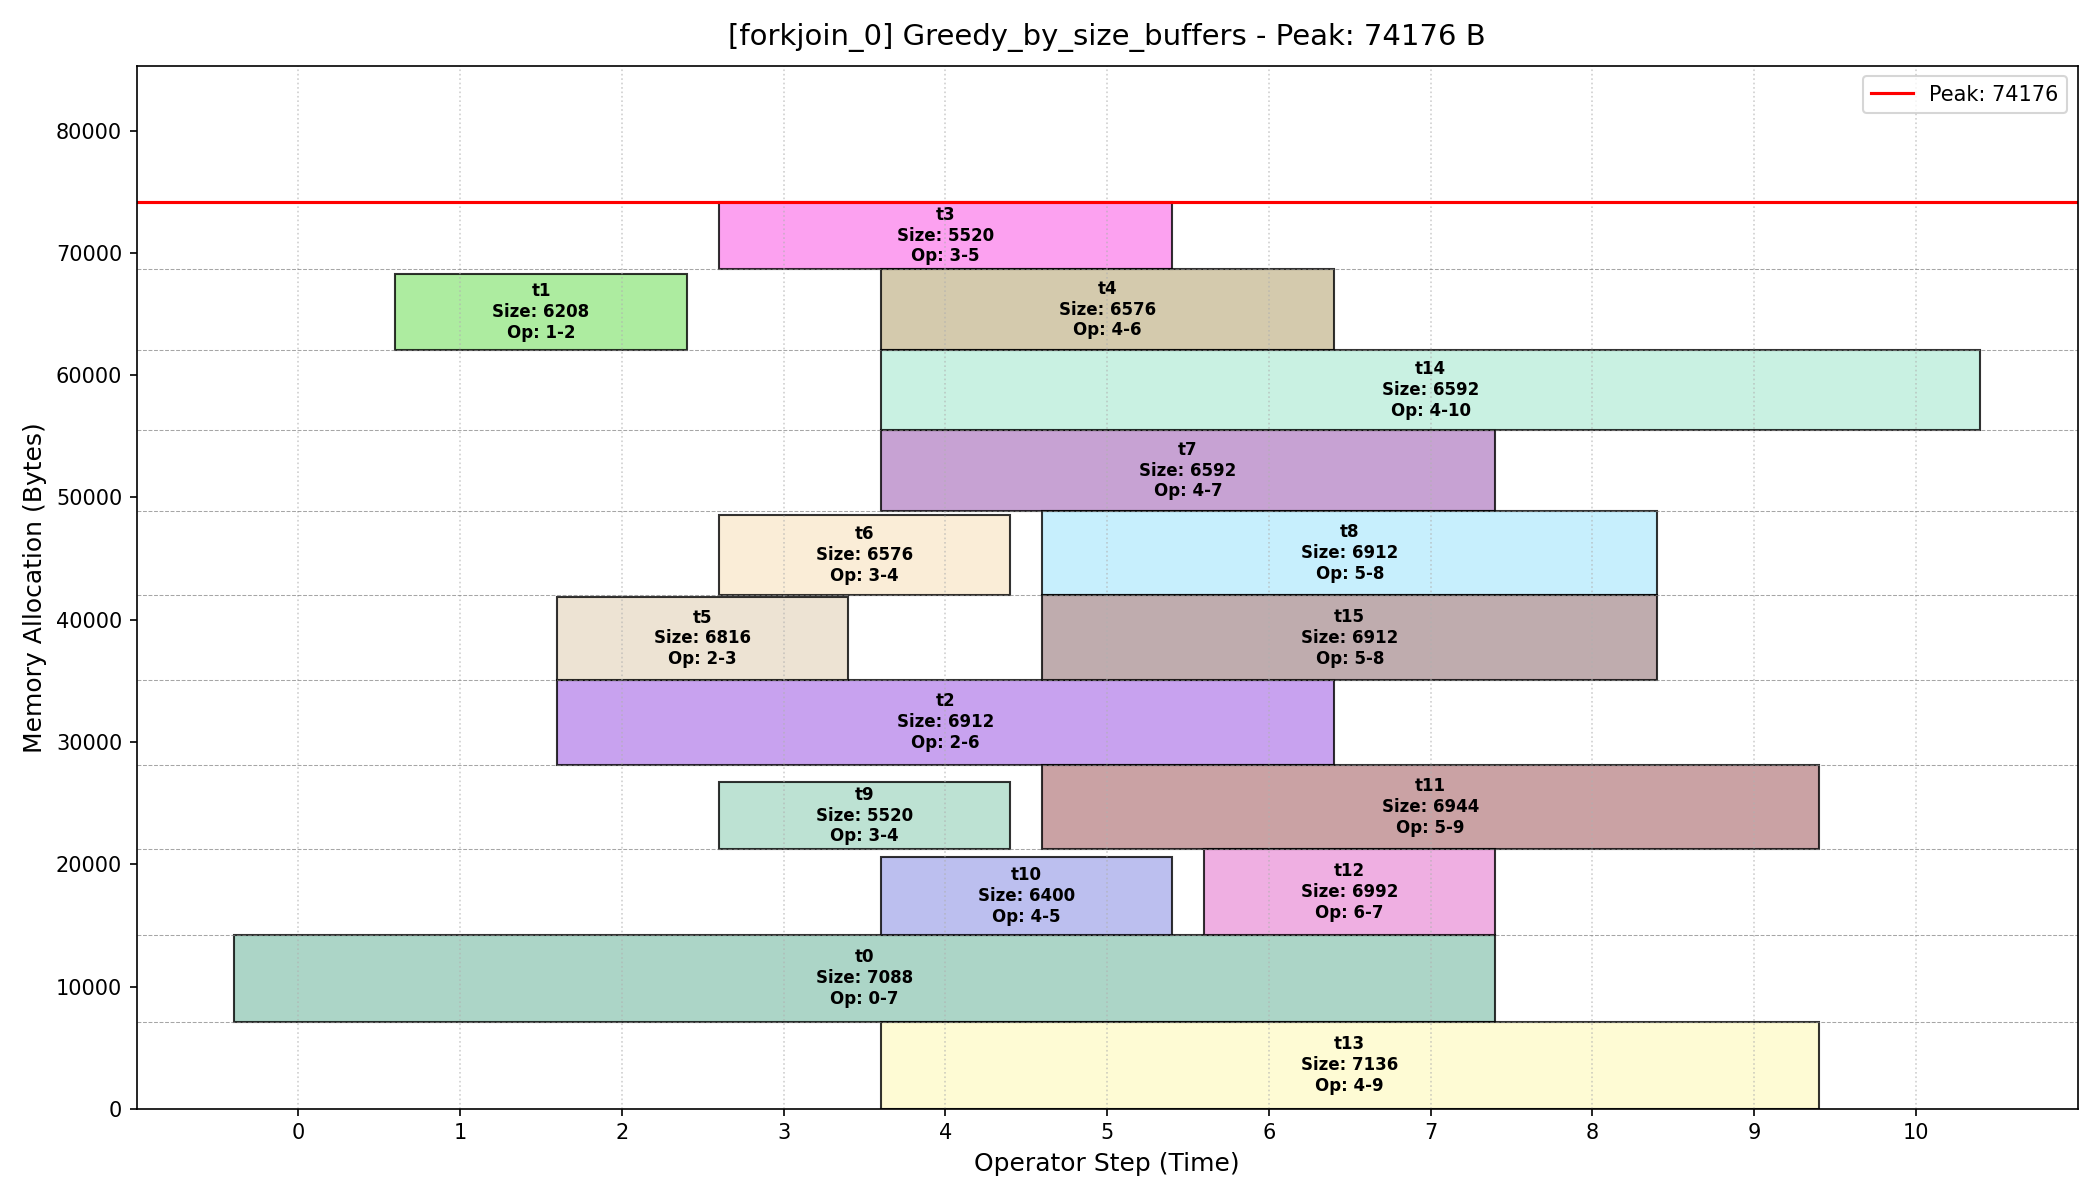
\includegraphics[width=1\textwidth]{figures/forkjoin_0_Greedy_by_size_buffers.png} \\
    \vspace{5pt}
    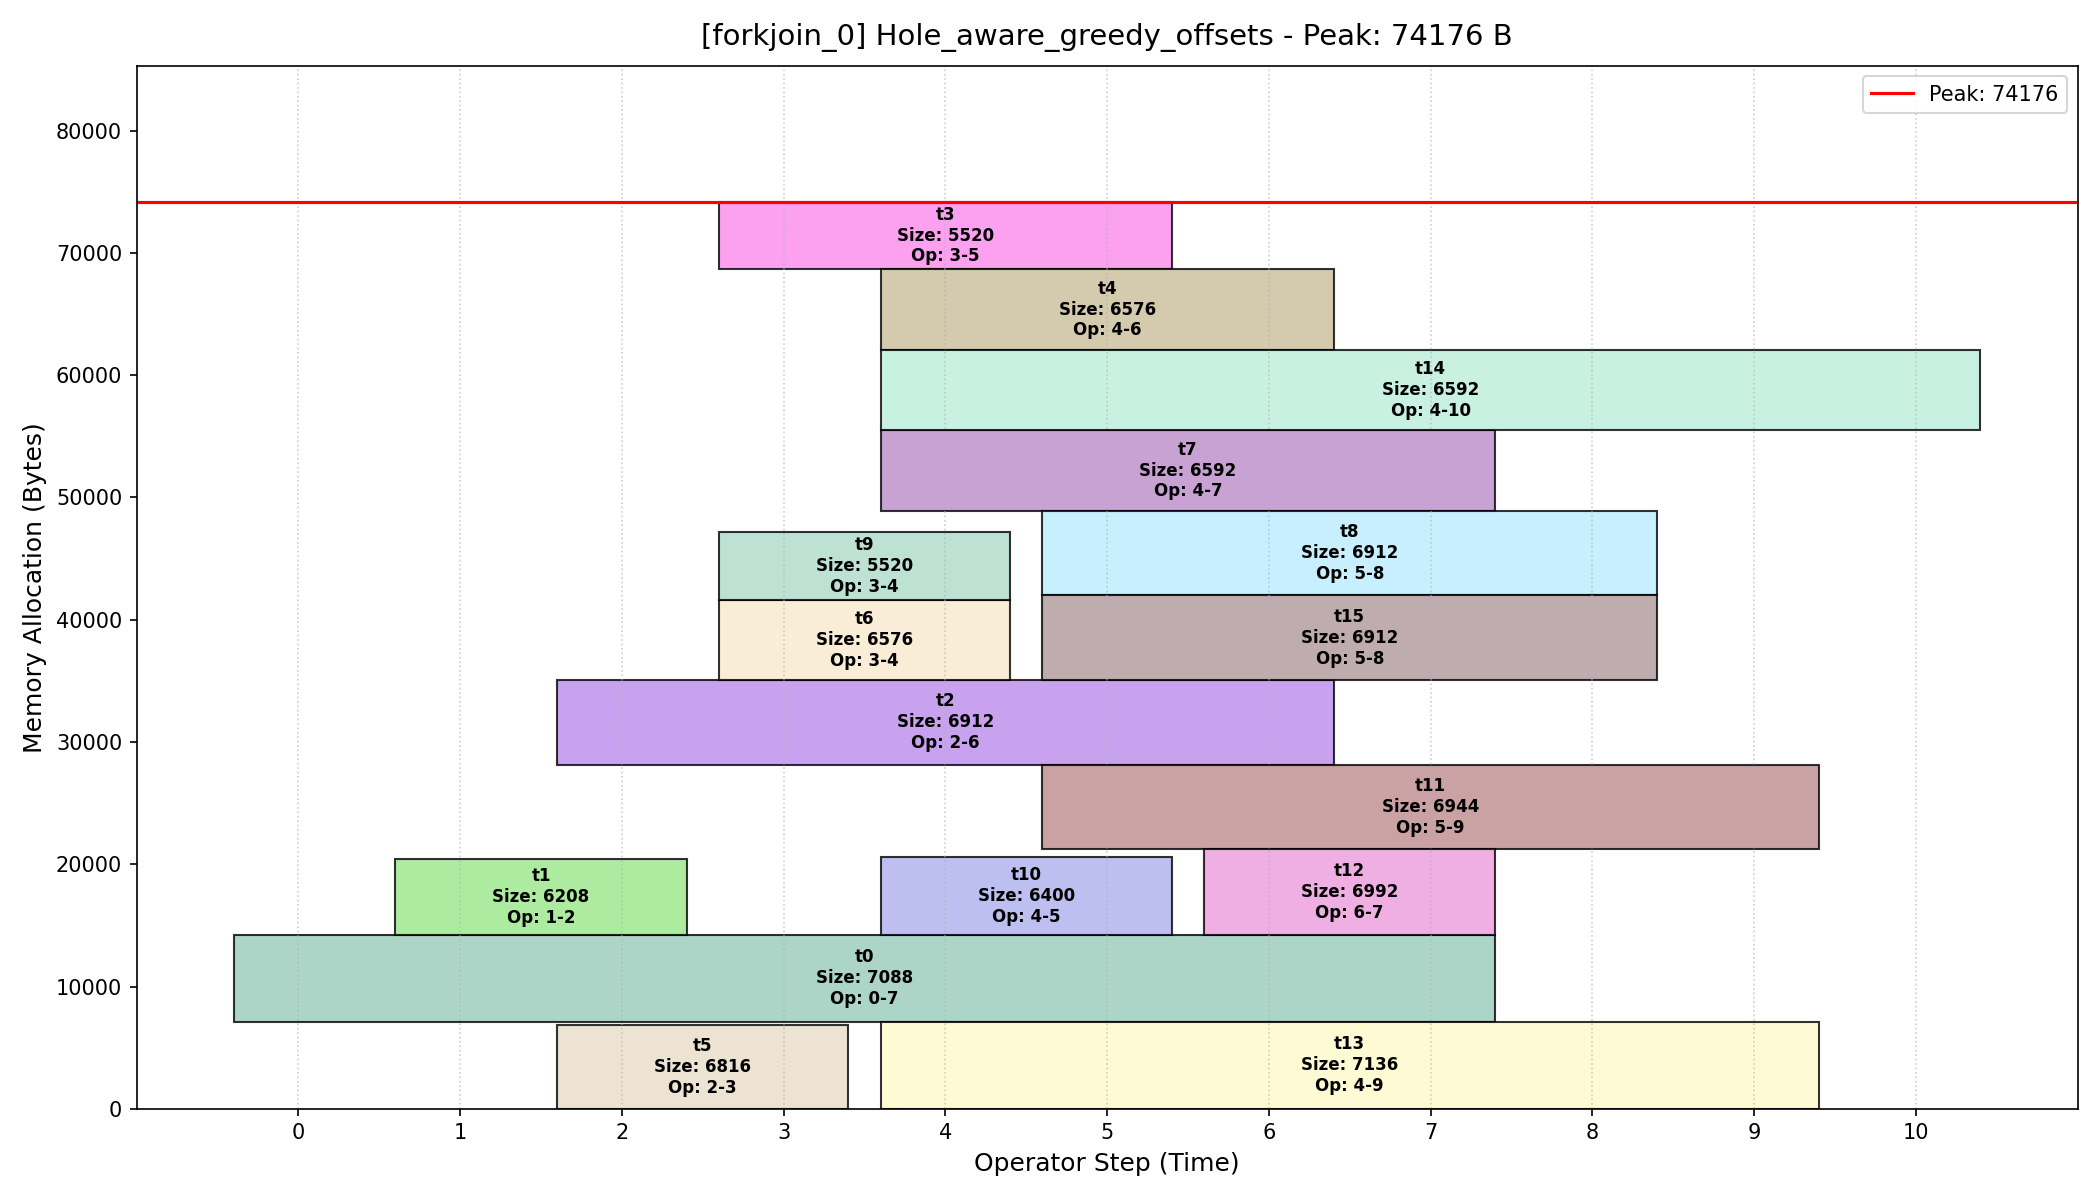
\includegraphics[width=1\textwidth]{figures/forkjoin_0_Hole_aware_greedy_offsets.png}
    \caption{Same Peak Memory Consumption but different allocation}
\end{figure}